\section{Plant considered for system identification} \label{sec:plant_considered}
    \begin{figure}[h]
        \centering
        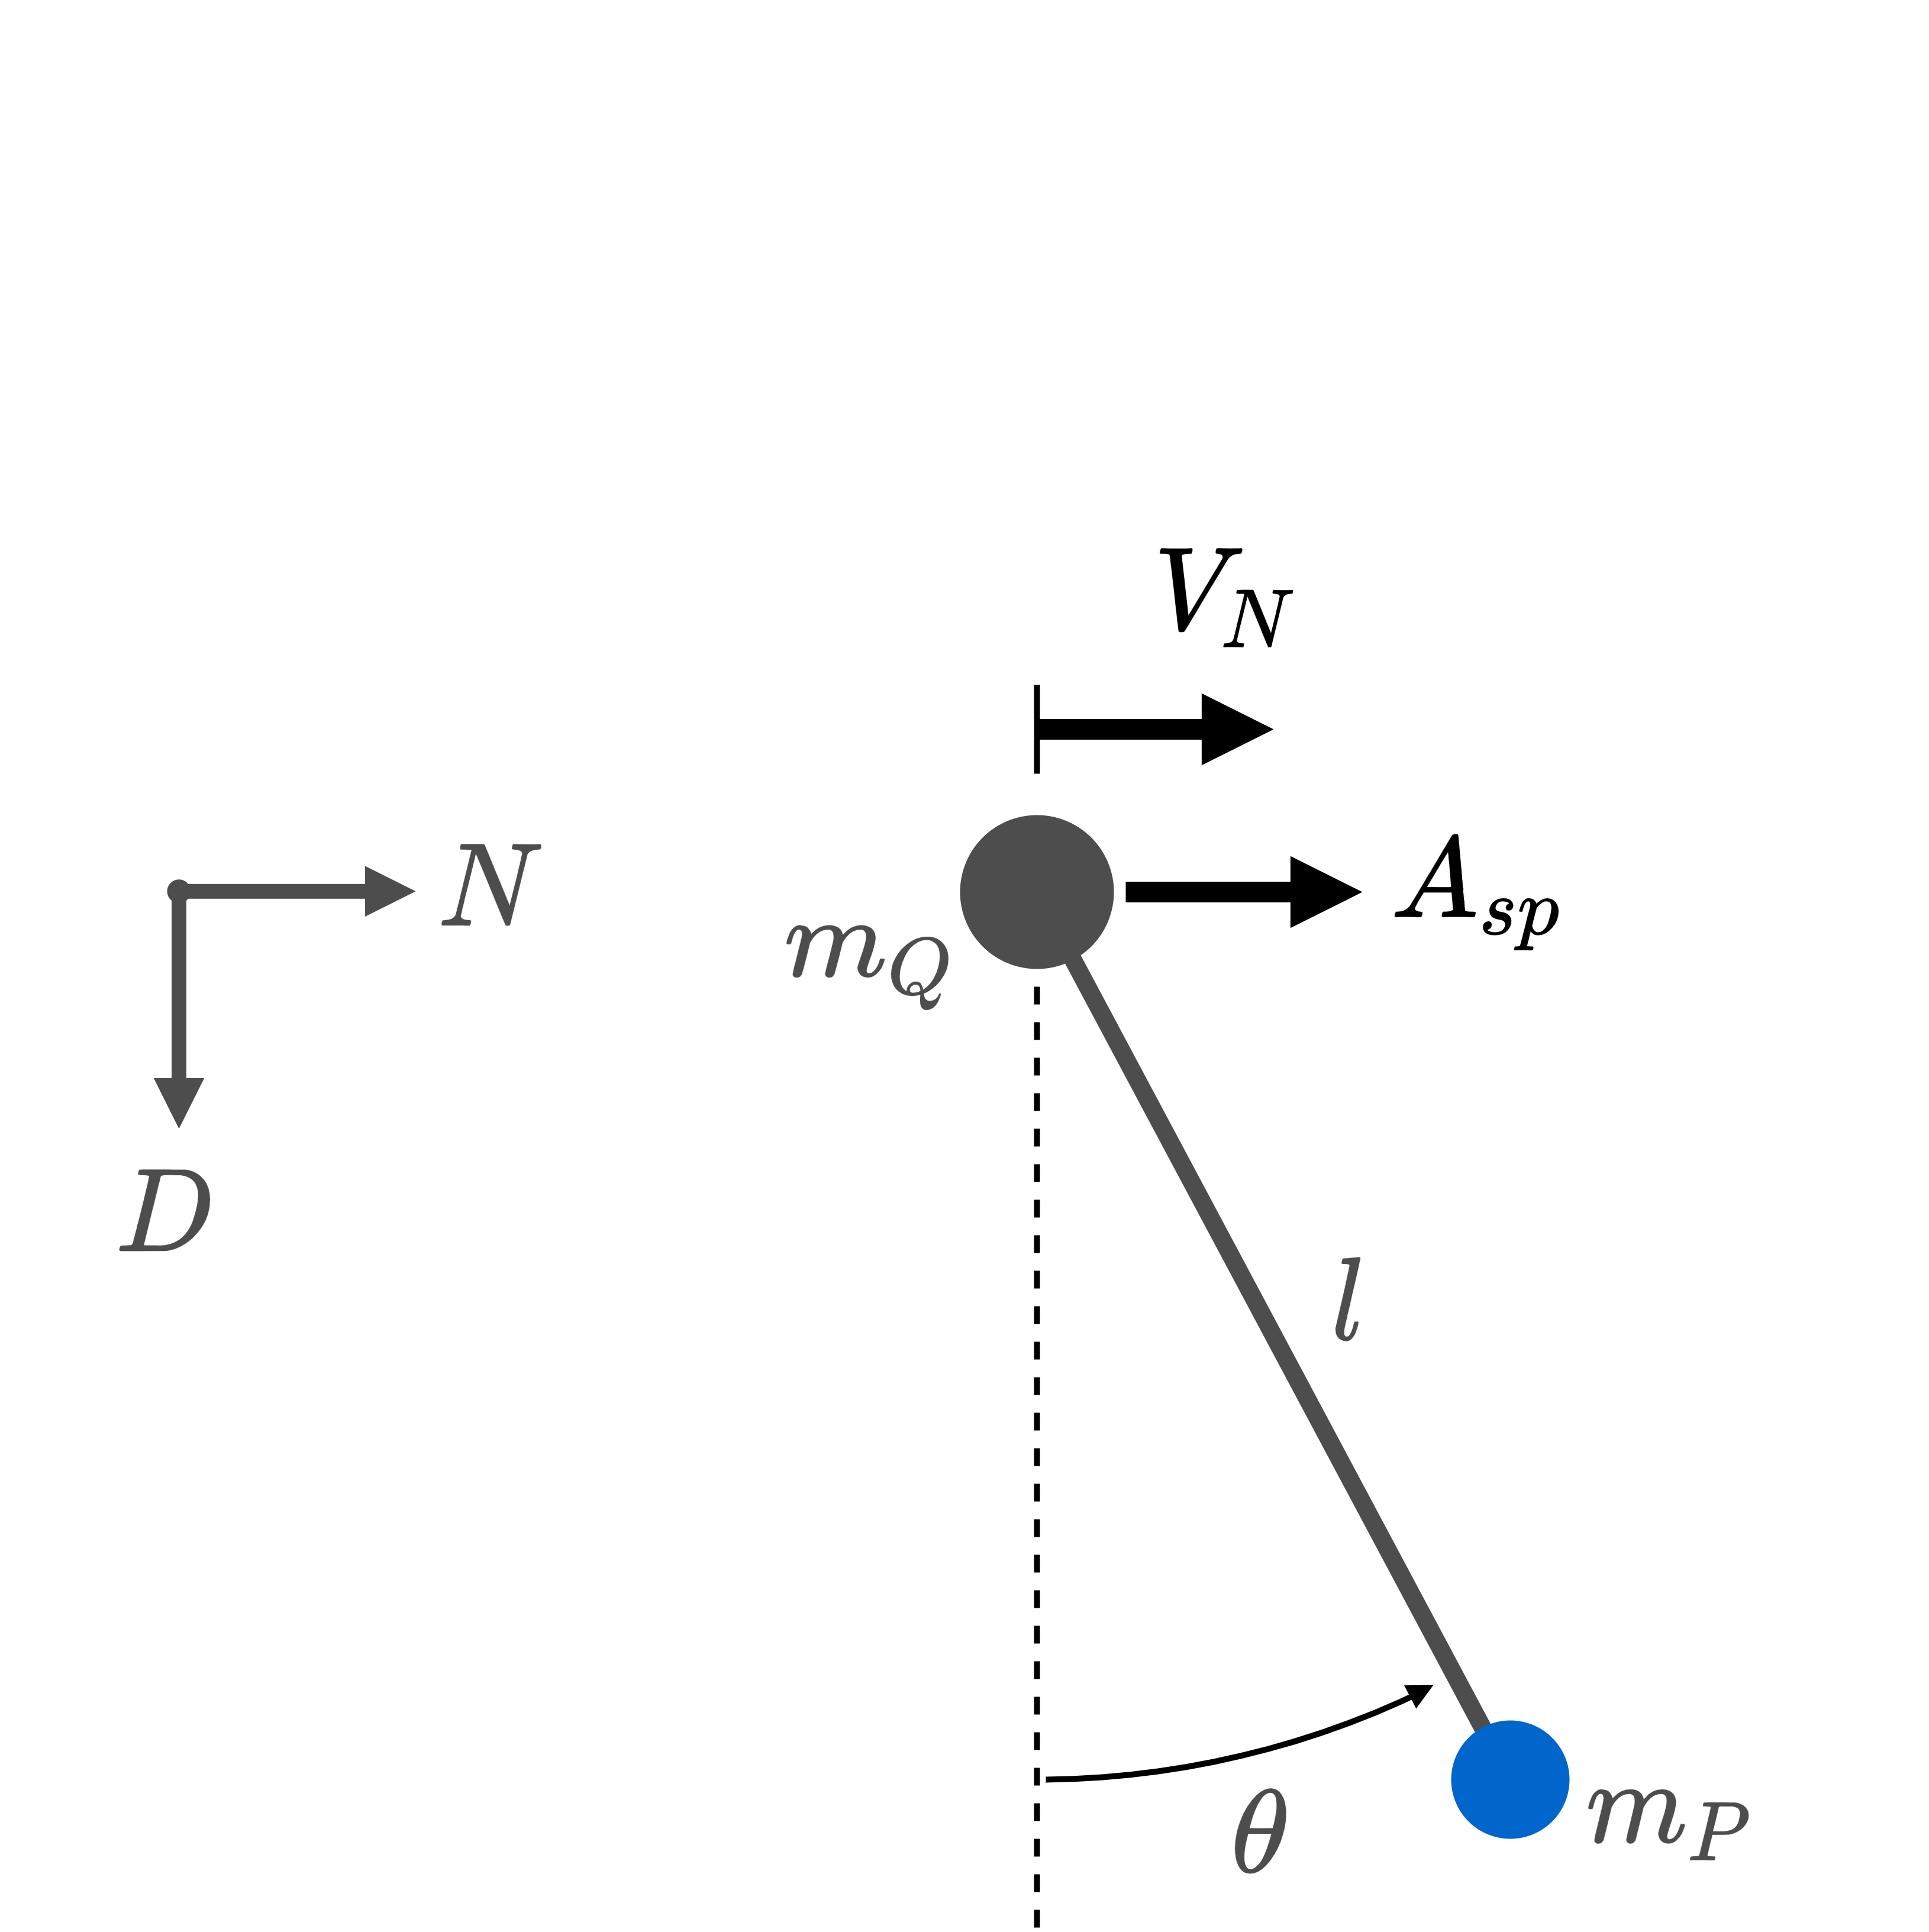
\includegraphics[width=0.5\linewidth]{floating_pend.png}            
        \caption{Floating pendulum model considered for system identification for a North velocity controller}
        \label{fig:floating_pend}
    \end{figure}

    \paragraph
    Figure \ref{fig:floating_pend} shows the plant considered for system identification.
    In Chapter~\ref{chap:modelling} the differential equations that describe the motion of this system are derived with Lagrangian mechanics.
    From these equations it is clear that the considered plant is defined by the state vector,
    \begin{equation}
        \bm{x} = \begin{bmatrix}
            V_N & \dot{\theta}
        \end{bmatrix}^T,
    \end{equation}
    and the input vector,
    \begin{equation}
        \bm{u} = \begin{bmatrix}
            A_{N,sp}
        \end{bmatrix},
    \end{equation}

    % From this derivation it is clear that the angular velocity of the payload, $\dot{\theta}$, is required to described the system dynamics.
    % However, $\dot{\theta}$ is not measured directly on the considered practical quadrotor setup.
    % Instead, the payload angle, $\theta$, is measured by a potentiometer attached to a ADC on Honeybee as described in Chapter \ref{chap:system_overview}.
    % As expected, this measurement is extremely noisy.
    % \murray{Maybe insert figure to show noise}
    % % Figure \ref{} shows the angle measurement during a practical experiment of the payload while Honeybee is held stationary
    % Numerical differentiation is applied to the noisy $\theta$ signal which results in a very inaccurate estimation of $\dot{\theta}$.
    % Therefore it is desirable to rather use $\theta$ in the system identification process. 

